\documentclass[11pt]{article}

\usepackage{setspace}
\usepackage{amsmath}
\usepackage{enumitem}
\usepackage{amsfonts} 
\usepackage{mathtools}
\usepackage{relsize}
\usepackage{graphicx}
\usepackage[top=2cm,bottom=2cm,left=2.5cm,right=2.5cm,marginparwidth=1.75cm]{geometry}
\setlength{\parindent}{0cm}
\usepackage{listings}
\usepackage{clrscode3e}
\usepackage{graphicx}

\title{\vspace{-1.0cm}PHYS 2303 Homework 5}
\author{Fletcher Gornick}
\date{February 20, 2022}

\spacing{1.5}
\begin{document}
 \maketitle
 \section*{Volume 1 Chapter 17 Problem 105}
  A string with a linear mass density of \(\mu = 0.0062\) kg/m is stretched between two 
  posts 1.30 m apart. The tension in the string is 150.00 N. The string oscillates and 
  produces a sound wave. A 1024-Hz tuning fork is struck and the beat frequency between 
  the two sources is 52.83 Hz. What are the possible frequency and wavelength of the 
  wave on the string?
 \newpage

 \section*{Volume 1 Chapter 17 Problem 117}
  Two eagles fly directly toward one another, the first at 15.0 m/s and the second at 
  20.0 m/s. Both screech, the first one emitting a frequency of 3200 Hz and the second 
  one emitting a frequency of 3800 Hz. What frequencies do they receive if the speed of 
  sound is 330 m/s?
 \newpage

 \section*{Volume 1 Chapter 17 Problem 141}
  Two speakers producing the same frequency of sound are a distance of \(d\) apart. 
  Consider an arc along a circle of radius \(R\), centered at the midpoint of the 
  speakers, as shown below. \\\\
  (a) At what angles will there be maxima? \\
  (b) At what angle will there be minima?
  \begin{wrapfigure}{1}{0.25\textwidth}
   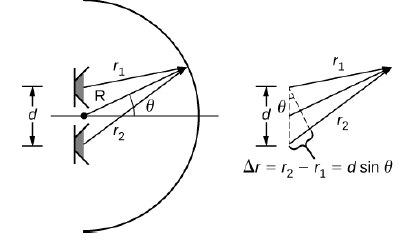
\includegraphics[scale=0.5]{1-17-141.png}
  \end{wrapfigure}
 \newpage

 \section*{Volume 3 Chapter 1 Problem 34}
  Suppose a man stands in front of a mirror as shown below. His eyes are 1.65 m above 
  the floor and the top of his head is 0.13 m higher. Find the height above the floor 
  of the top and bottom of the smallest mirror in which he can see both the top of his 
  head and his feet. How is this distance related to the man’s height? \\\\
  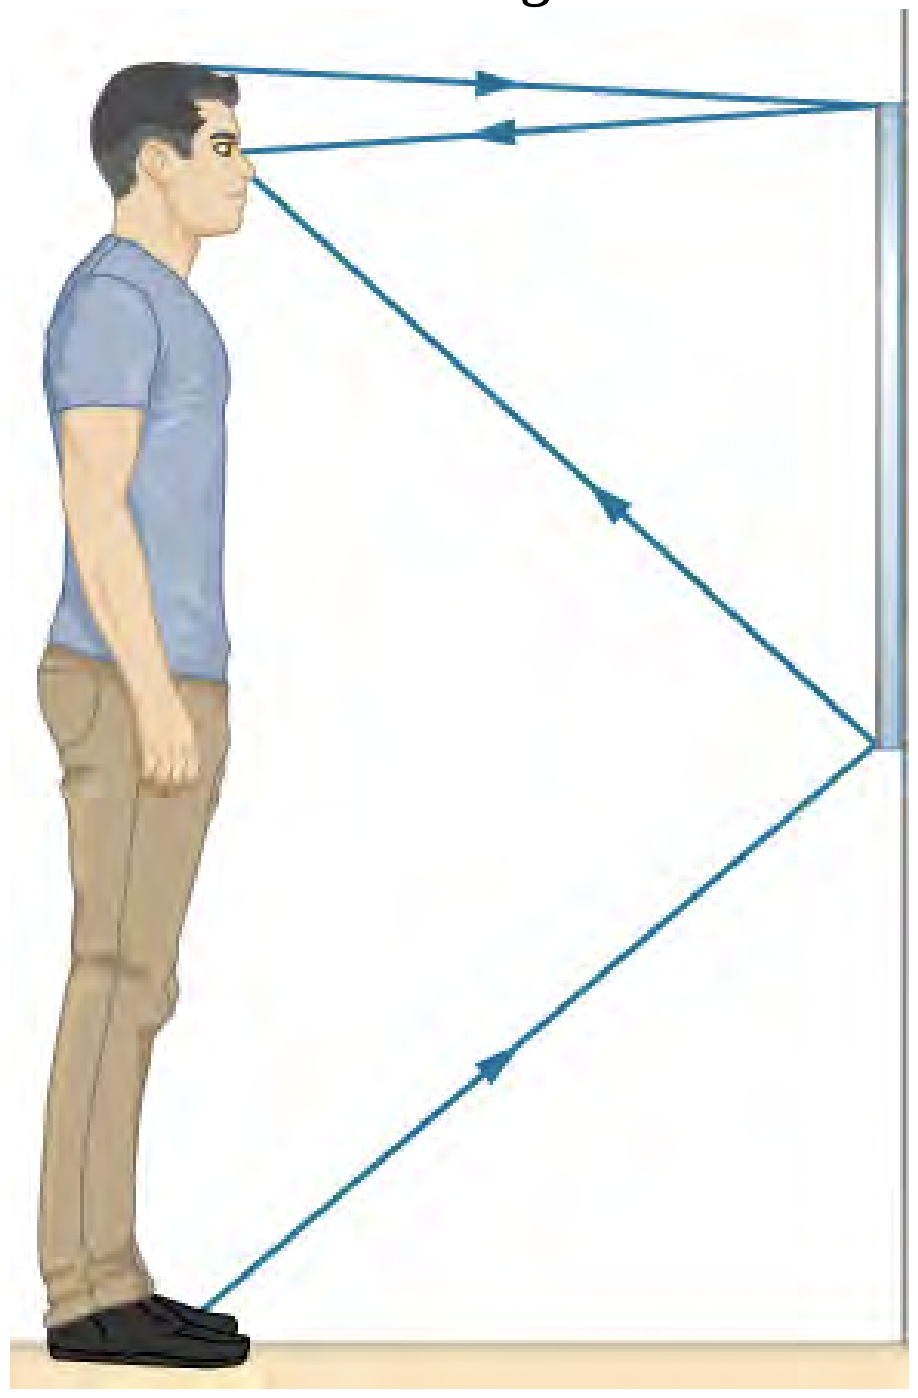
\includegraphics[scale=0.35]{3-1-34.png}
 \newpage

 \section*{Volume 3 Chapter 1 Problem 44}
  A scuba diver training in a pool looks at his instructor as shown below. What angle 
  does the ray from the instructor’s face make with the perpendicular to the water at 
  the point where the ray enters? The angle between the ray in the water and the 
  perpendicular to the water is 25.0\(^\circ\). \\\\
  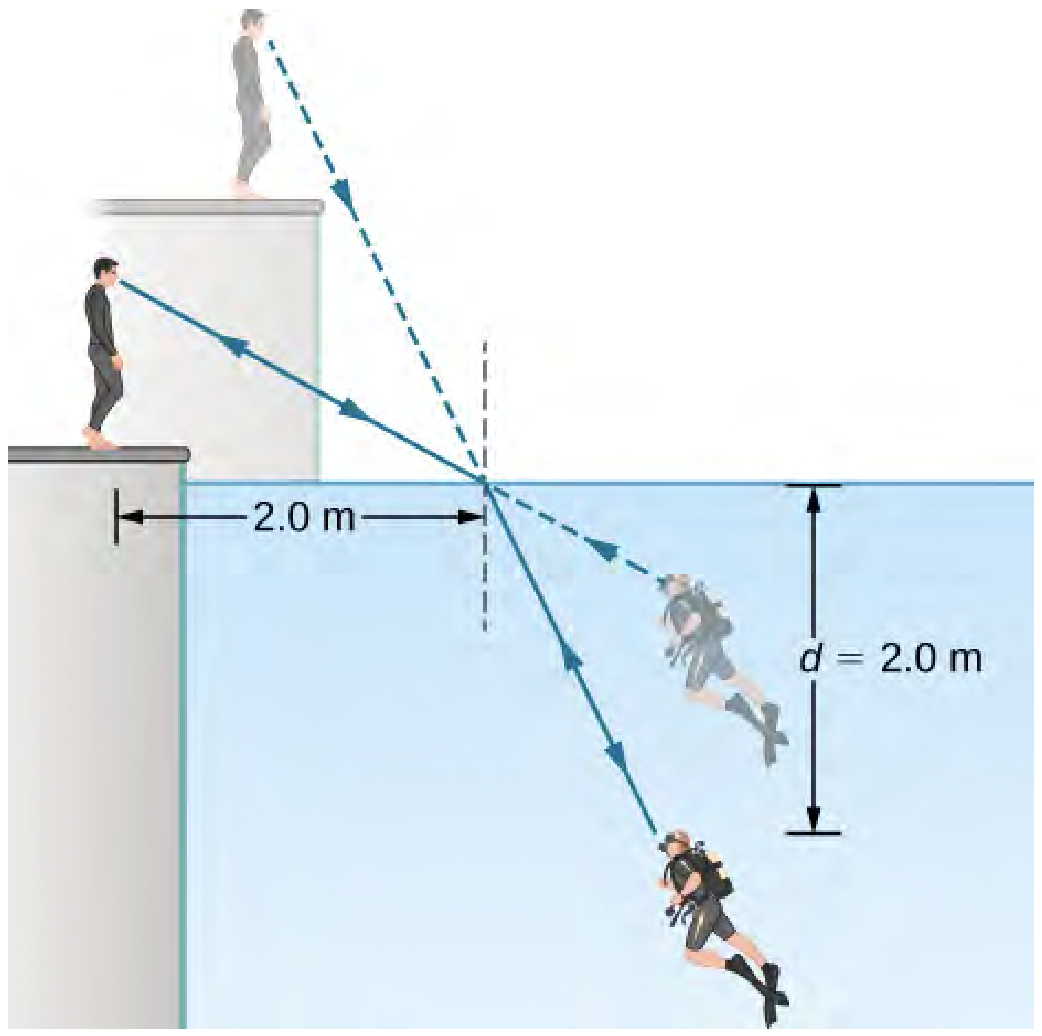
\includegraphics[scale=0.4]{3-1-44.png}

\end{document}

